\section{Wireless 802.15.4 (static)}
\subsection{Description of the simulation}
The simulation is based on the IEEE 802.15.4(static) standard. Routing is based on the dsdv protocol. The simulation is based on the ns-2 simulator. The simulation is based on the following parameters:
\begin{itemize}
    \item Channel: Wireless channel
    \item Propagation: Two-ray ground
    \item Antenna: Omnidirectional
    \item Link: 802.15.4
    \item Queue: Drop-tail
    \item Routing: DSDV
    \item Mobility: Static
    \item Position: Grid
    \item Area: 2*(tx\_range)m x 2*(tx\_range)m
    \item Flow: Random source to random destination
    \item Packet size: 64 bytes
    \item Number of nodes: Variable
    \item Number of flows: Variable
    \item Packet rate: Variable
    \item Tx Coverage: Variable
    \item Simulation time: 60 seconds
\end{itemize}

\subsection{Results}
\subsubsection{Varying Number of Nodes}
Baseline parameters are as follows:
\begin{itemize}
    \item Number of flows: 20
    \item Packet rate: 100 packets per second
    \item Tx Coverage: 300m
\end{itemize}
The number of nodes is varied from 20 to 100 in steps of 20.
See Figure \ref{node_throughput} ,\ref{node_delay} , \ref{node_delivery} , \ref{node_drop}, \ref{node_energy} , \ref{node_energy_per_byte} and \ref{node_per_node_throughput} for the result.
\begin{figure}[h]
\begin{subfigure}{.5\textwidth}
  \centering
  % include first image
  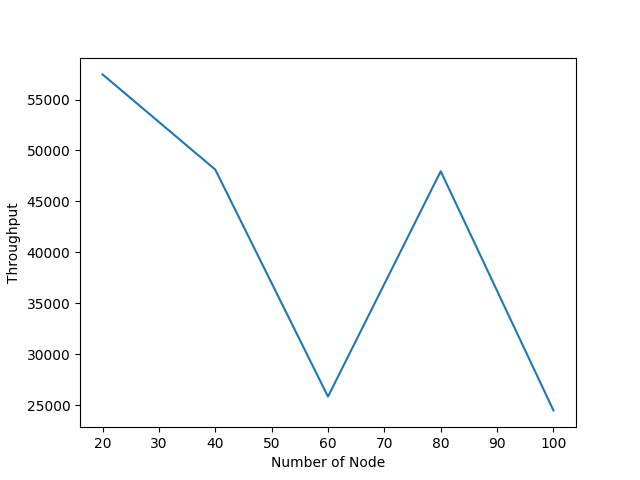
\includegraphics[width=.8\linewidth]{_15_4_static/NumberofNodevsThroughput.png}
     \caption{Number of Nodes Vs Throughput}
    \label{node_throughput}
\end{subfigure}
\begin{subfigure}{.5\textwidth}
  \centering
  % include second image
  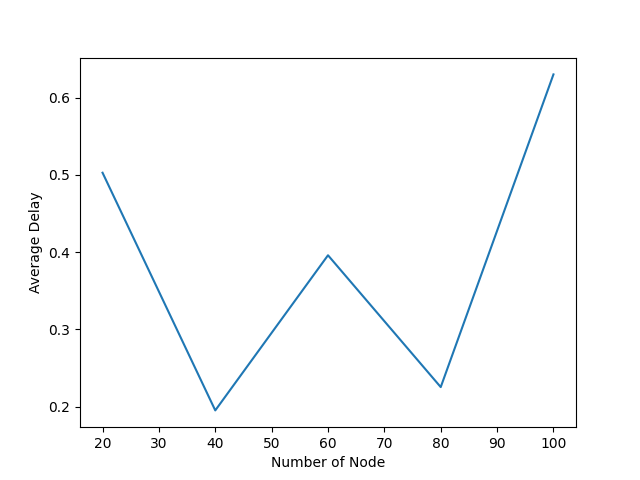
\includegraphics[width=.8\linewidth]{_15_4_static/NumberofNodevsAverageDelay.png}
    \caption{Number of Nodes Vs Average Delay}
     \label{node_delay}
\end{subfigure}
\begin{subfigure}{.5\textwidth}
  \centering
  % include third image
  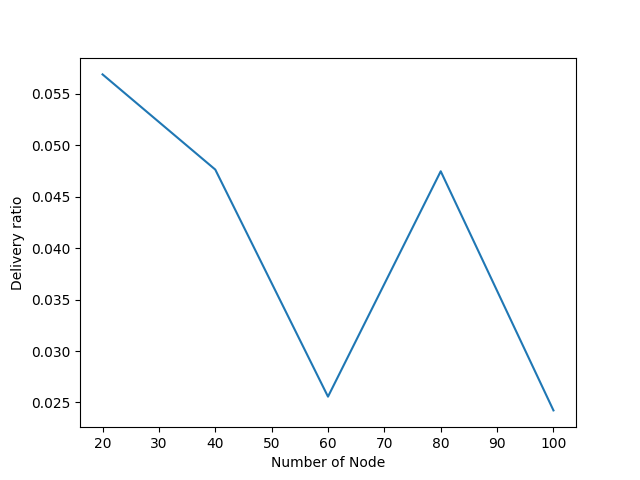
\includegraphics[width=.8\linewidth]{_15_4_static/NumberofNodevsDeliveryRatio.png}
     \caption{Number of Nodes Vs Delivary Ratio}
     \label{node_delivery}
\end{subfigure}
\begin{subfigure}{.5\textwidth}
  \centering
  % include fourth image
  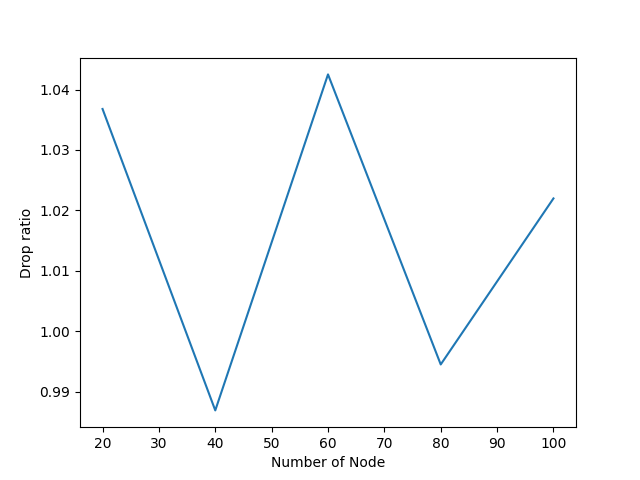
\includegraphics[width=.8\linewidth]{_15_4_static/NumberofNodevsDropRatio.png}
     \caption{Number of Nodes Vs Drop Ratio}
     \label{node_drop}
\end{subfigure}
\begin{subfigure}{.5\textwidth}
  \centering
  % include fifth image
  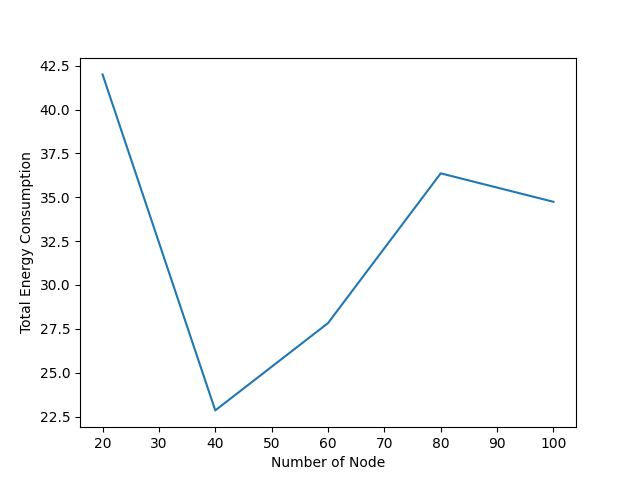
\includegraphics[width=.8\linewidth]{_15_4_static/NumberofNodevsTotalEnergyConsumption.png}
     \caption{Number of Nodes Vs Energy Consumption}
     \label{node_energy}
\end{subfigure}
\begin{subfigure}{.5\textwidth}
  \centering
  % include sixth image
  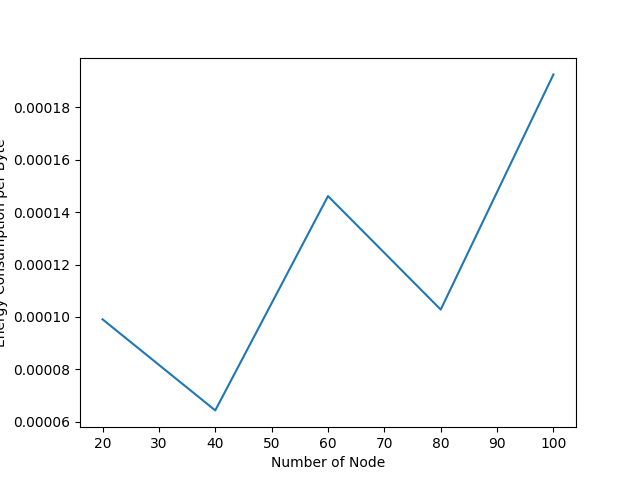
\includegraphics[width=.8\linewidth]{_15_4_static/NumberofNodevsEnergyConsumptionperByte.png}
     \caption{Number of Nodes Vs Energy Per Byte}
     \label{node_energy_per_byte}
\end{subfigure}
\caption{Varying Number of Nodes}
\label{fig:varyingNode}
\end{figure}
\begin{figure}[h]
\begin{subfigure}{.5\textwidth}
  \centering
  % include first image
  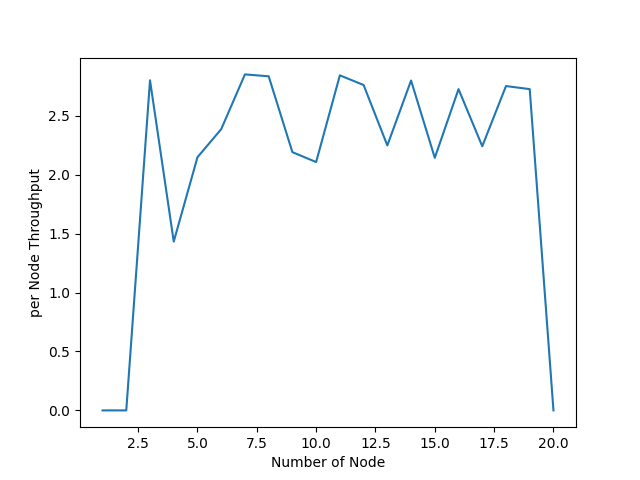
\includegraphics[width=.8\linewidth]{_15_4_static/NumberofNode(20)vsperNodeThroughput.png}
     \caption{Number of Nodes(20) Vs Throughput per Node}
 \end{subfigure}
\begin{subfigure}{.5\textwidth}
  \centering
  % include second image
  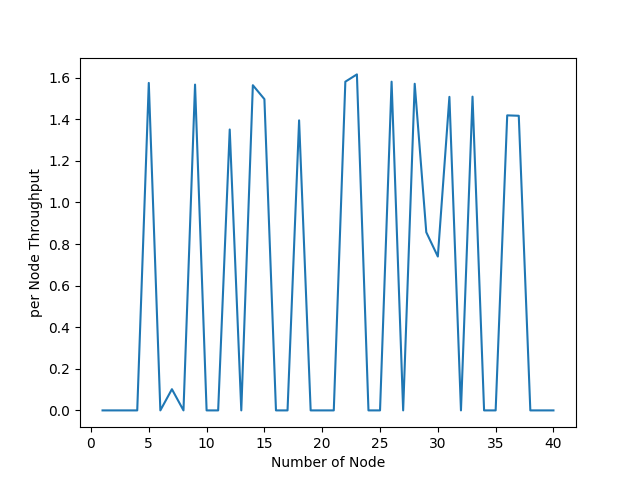
\includegraphics[width=.8\linewidth]{_15_4_static/NumberofNode(40)vsperNodeThroughput.png}
     \caption{Number of Nodes(40) Vs Throughput per Node}
    \end{subfigure}
\begin{subfigure}{.5\textwidth}
    \centering
    % include third image
    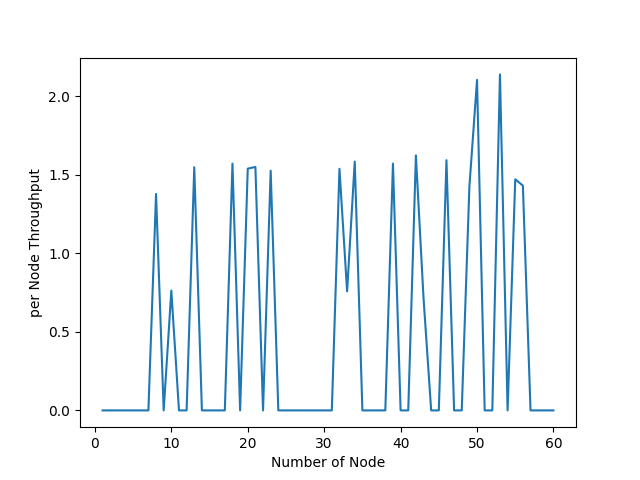
\includegraphics[width=.8\linewidth]{_15_4_static/NumberofNode(60)vsperNodeThroughput.png}
         \caption{Number of Nodes(60) Vs Throughput per Node}
        \end{subfigure}
\begin{subfigure}{.5\textwidth}
    \centering
    % include fourth image
    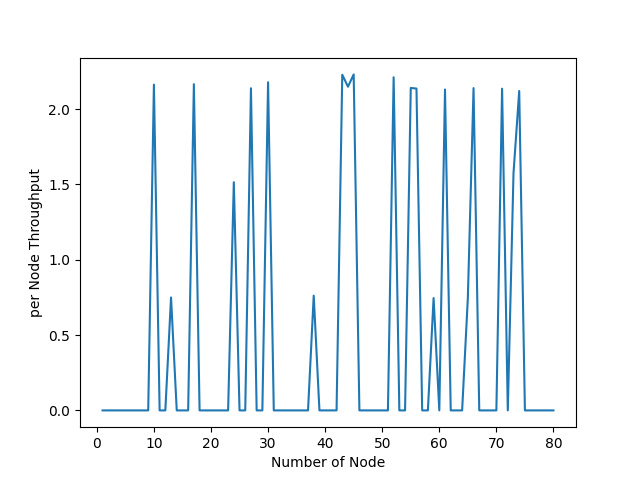
\includegraphics[width=.8\linewidth]{_15_4_static/NumberofNode(80)vsperNodeThroughput.png}
         \caption{Number of Nodes(80) Vs Throughput per Node}
        \end{subfigure}
\begin{subfigure}{.5\textwidth}
    \centering
    % include fifth image
    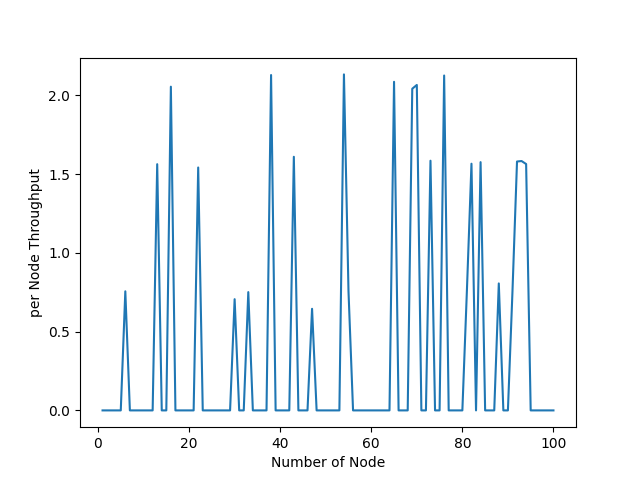
\includegraphics[width=.8\linewidth]{_15_4_static/NumberofNode(100)vsperNodeThroughput.png}
         \caption{Number of Nodes(100) Vs Throughput per Node}
        \end{subfigure}
\caption{Varying Number of Nodes (Throughput per Node)}
\label{node_per_node_throughput}
\end{figure}

\subsubsection{Varying Number of Flows}
Baseline parameters are as follows:
\begin{itemize}
    \item Number of nodes: 40
    \item Packet rate: 100 packets per second
    \item Tx Coverage: 300m
\end{itemize}
The number of flows is varied from 10 to 50 in steps of 10.
See Figure \ref{flow_throughput} ,\ref{flow_delay} , \ref{flow_delivery} , \ref{flow_drop}, \ref{flow_energy} , \ref{flow_energy_per_byte} and \ref{flow_per_node_throughput} for the result.
\begin{figure}[h]
\begin{subfigure}{.5\textwidth}
  \centering
  % include first image
  \includegraphics[width=.8\linewidth]{_15_4_static/NumberofFlowvsThroughput.png}
     \caption{Number of Flows Vs Throughput}
    \label{flow_throughput}
\end{subfigure}
\begin{subfigure}{.5\textwidth}
  \centering
  % include second image
  \includegraphics[width=.8\linewidth]{_15_4_static/NumberofFlowvsAverageDelay.png}
    \caption{Number of Flows Vs Average Delay}
     \label{flow_delay}
\end{subfigure}
\begin{subfigure}{.5\textwidth}
  \centering
  % include third image
  \includegraphics[width=.8\linewidth]{_15_4_static/NumberofFlowvsDeliveryRatio.png}
     \caption{Number of Flows Vs Delivary Ratio}
     \label{flow_delivery}
\end{subfigure}
\begin{subfigure}{.5\textwidth}
  \centering
  % include fourth image
  \includegraphics[width=.8\linewidth]{_15_4_static/NumberofFlowvsDropRatio.png}
     \caption{Number of Flows Vs Drop Ratio}
     \label{flow_drop}
\end{subfigure}
\begin{subfigure}{.5\textwidth}
  \centering
  % include fifth image
  \includegraphics[width=.8\linewidth]{_15_4_static/NumberofFlowvsTotalEnergyConsumption.png}
     \caption{Number of Flows Vs Energy Consumption}
     \label{flow_energy}
\end{subfigure}
\begin{subfigure}{.5\textwidth}
  \centering
  % include sixth image
  \includegraphics[width=.8\linewidth]{_15_4_static/NumberofFlowvsEnergyConsumptionperByte.png}
     \caption{Number of Flows Vs Energy Per Byte}
     \label{flow_energy_per_byte}
\end{subfigure}
\caption{Varying Number of Flows}
\label{fig:varyingFlow}
\end{figure}
\begin{figure}[h]
\begin{subfigure}{.5\textwidth}
  \centering
  % include first image
  \includegraphics[width=.8\linewidth]{_15_4_static/NumberofFlow(10)vsperNodeThroughput.png}
     \caption{Number of Flows(10) Vs Throughput per Node}
 \end{subfigure}
\begin{subfigure}{.5\textwidth}
  \centering
  % include second image
  \includegraphics[width=.8\linewidth]{_15_4_static/NumberofFlow(20)vsperNodeThroughput.png}
     \caption{Number of Flows(20) Vs Throughput per Node}
    \end{subfigure}
\begin{subfigure}{.5\textwidth}
    \centering
    % include third image
    \includegraphics[width=.8\linewidth]{_15_4_static/NumberofFlow(30)vsperNodeThroughput.png}
         \caption{Number of Flows(30) Vs Throughput per Node}
        \end{subfigure}
\begin{subfigure}{.5\textwidth}
    \centering
    % include fourth image
    \includegraphics[width=.8\linewidth]{_15_4_static/NumberofFlow(40)vsperNodeThroughput.png}
         \caption{Number of Flows(40) Vs Throughput per Node}
        \end{subfigure}
\begin{subfigure}{.5\textwidth}
    \centering
    % include fifth image
    \includegraphics[width=.8\linewidth]{_15_4_static/NumberofFlow(50)vsperNodeThroughput.png}
         \caption{Number of Flows(50) Vs Throughput per Node}
        \end{subfigure}
\caption{Varying Number of Flows (Throughput per Node)}
\label{flow_per_node_throughput}
\end{figure}

\subsubsection{Varying Packet per Second}
Baseline parameters are as follows:
\begin{itemize}
    \item Number of nodes: 40
    \item Number of flows: 10
    \item Tx Coverage: 300m
\end{itemize}
The packet rate is varied from 100 to 500 packets per second in steps of 100.
See Figure \ref{packet_rate_throughput} ,\ref{packet_rate_delay} , \ref{packet_rate_delivery} , \ref{packet_rate_drop}, \ref{packet_rate_energy} , \ref{packet_rate_energy_per_byte} and \ref{packet_rate_per_node_throughput} for the result.
\begin{figure}[h]
\begin{subfigure}{.5\textwidth}
  \centering
  % include first image
  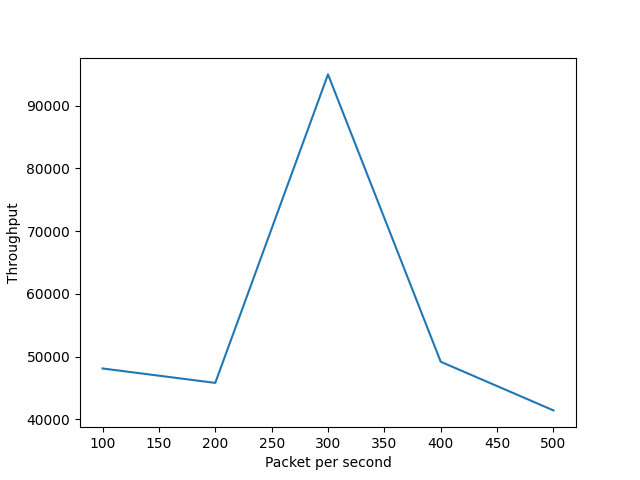
\includegraphics[width=.8\linewidth]{_15_4_static/PacketpersecondvsThroughput.png}
     \caption{Packet Rate Vs Throughput}
    \label{packet_rate_throughput}
\end{subfigure}
\begin{subfigure}{.5\textwidth}
  \centering
  % include second image
  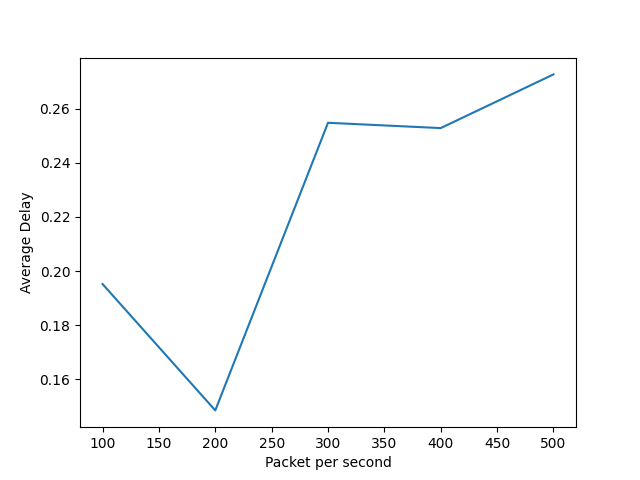
\includegraphics[width=.8\linewidth]{_15_4_static/PacketpersecondvsAverageDelay.png}
    \caption{Packet Rate Vs Average Delay}
     \label{packet_rate_delay}
\end{subfigure}
\begin{subfigure}{.5\textwidth}
  \centering
  % include third image
  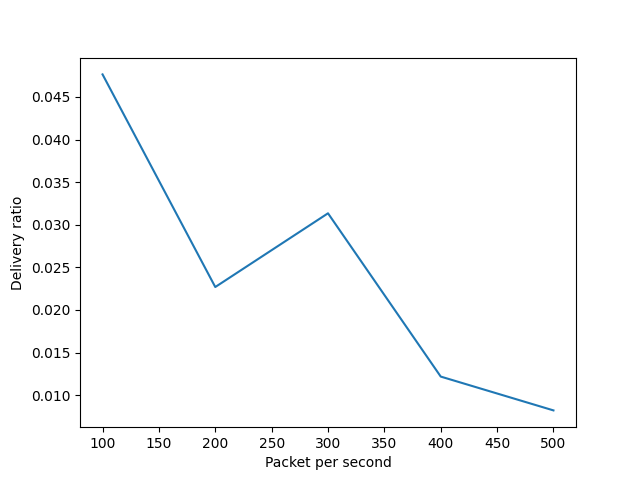
\includegraphics[width=.8\linewidth]{_15_4_static/PacketpersecondvsDeliveryRatio.png}
     \caption{Packet Rate Vs Delivary Ratio}
     \label{packet_rate_delivery}
\end{subfigure}
\begin{subfigure}{.5\textwidth}
  \centering
  % include fourth image
  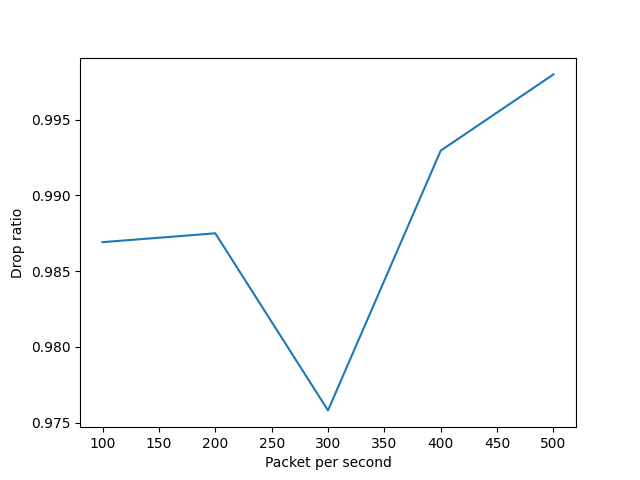
\includegraphics[width=.8\linewidth]{_15_4_static/PacketpersecondvsDropRatio.png}
     \caption{Packet Rate Vs Drop Ratio}
     \label{packet_rate_drop}
\end{subfigure}
\begin{subfigure}{.5\textwidth}
  \centering
  % include fifth image
  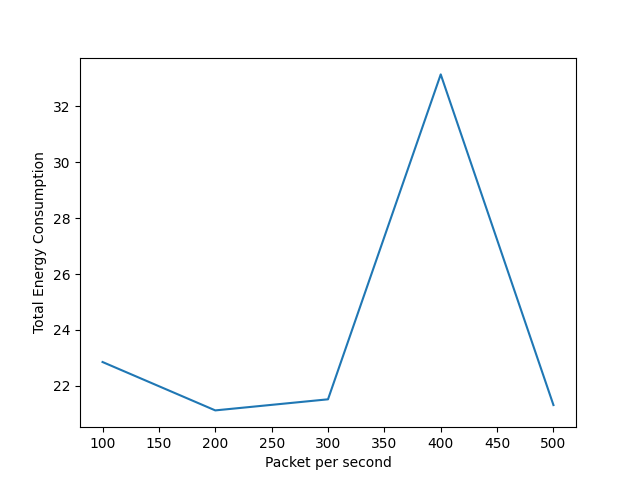
\includegraphics[width=.8\linewidth]{_15_4_static/PacketpersecondvsTotalEnergyConsumption.png}
     \caption{Packet Rate Vs Energy Consumption}
     \label{packet_rate_energy}
\end{subfigure}
\begin{subfigure}{.5\textwidth}
  \centering
  % include sixth image
  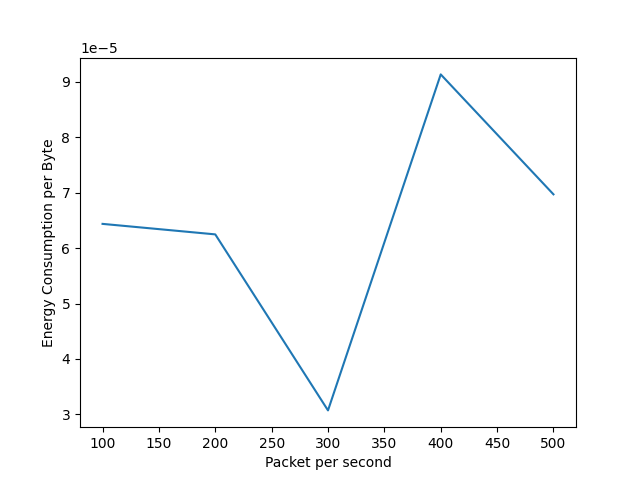
\includegraphics[width=.8\linewidth]{_15_4_static/PacketpersecondvsEnergyConsumptionperByte.png}
     \caption{Packet Rate Vs Energy Per Byte}
     \label{packet_rate_energy_per_byte}
\end{subfigure}
\caption{Varying Packet Rate}
\label{fig:varyingPacketRate}
\end{figure}
\begin{figure}[h]
\begin{subfigure}{.5\textwidth}
  \centering
  % include first image
  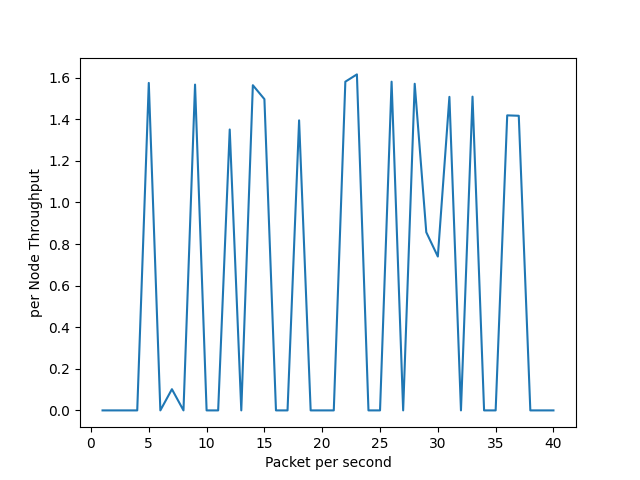
\includegraphics[width=.8\linewidth]{_15_4_static/Packetpersecond(100)vsperNodeThroughput.png}
     \caption{Packet Rate(100) Vs Throughput per Node}
 \end{subfigure}
\begin{subfigure}{.5\textwidth}
  \centering
  % include second image
  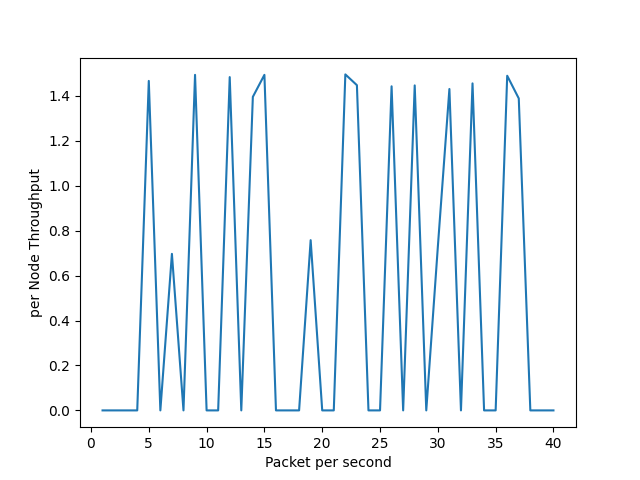
\includegraphics[width=.8\linewidth]{_15_4_static/Packetpersecond(200)vsperNodeThroughput.png}
     \caption{Packet Rate(200) Vs Throughput per Node}
    \end{subfigure}
\begin{subfigure}{.5\textwidth}
    \centering
    % include third image
    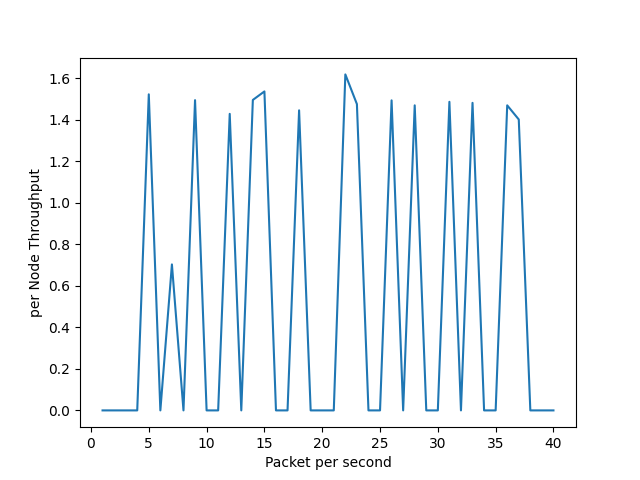
\includegraphics[width=.8\linewidth]{_15_4_static/Packetpersecond(300)vsperNodeThroughput.png}
         \caption{Packet Rate(300) Vs Throughput per Node}
        \end{subfigure}
\begin{subfigure}{.5\textwidth}
    \centering
    % include fourth image
    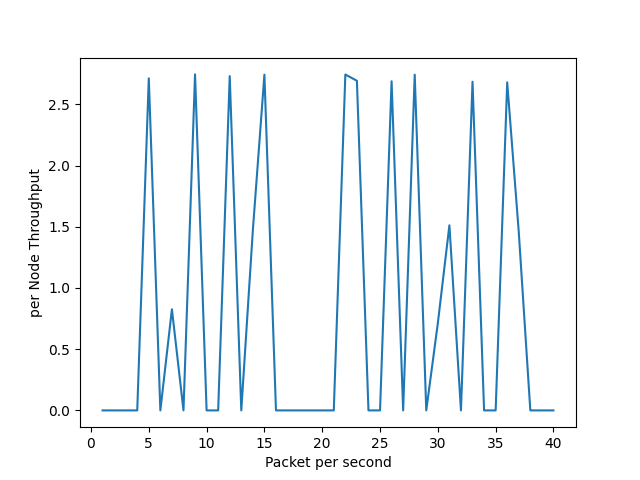
\includegraphics[width=.8\linewidth]{_15_4_static/Packetpersecond(400)vsperNodeThroughput.png}
         \caption{Packet Rate(400) Vs Throughput per Node}
        \end{subfigure}
\begin{subfigure}{.5\textwidth}
    \centering
    % include fifth image
    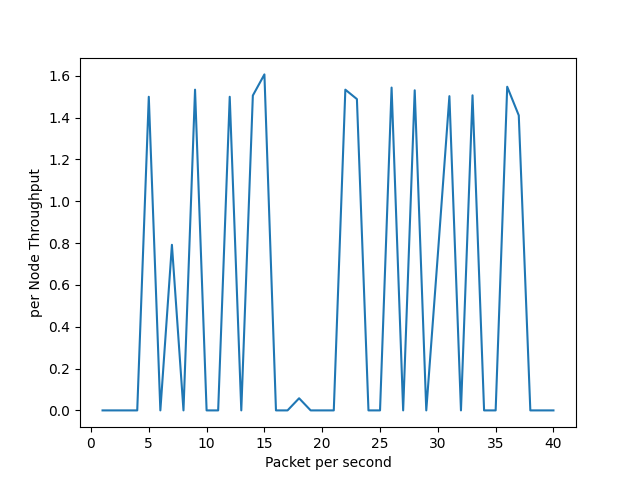
\includegraphics[width=.8\linewidth]{_15_4_static/Packetpersecond(500)vsperNodeThroughput.png}
         \caption{Packet Rate(500) Vs Throughput per Node}
        \end{subfigure}
\caption{Varying Packet Rate (Throughput per Node)}
\label{packet_rate_per_node_throughput}
\end{figure}
\subsubsection{Varying Transmission Range}
Baseline parameters are as follows:
\begin{itemize}
    \item Number of nodes: 40
    \item Number of flows: 10
    \item Packet Rate: 100 packets per second
\end{itemize}
The transmission range is varied from 100 to 500 meters in steps of 100.
See Figure \ref{tx_range_throughput} ,\ref{tx_range_delay} , \ref{tx_range_delivery} , \ref{tx_range_drop}, \ref{tx_range_energy} , \ref{tx_range_energy_per_byte} and \ref{tx_range_per_node_throughput} for the result.
\begin{figure}[h]
\begin{subfigure}{.5\textwidth}
  \centering
  % include first image
  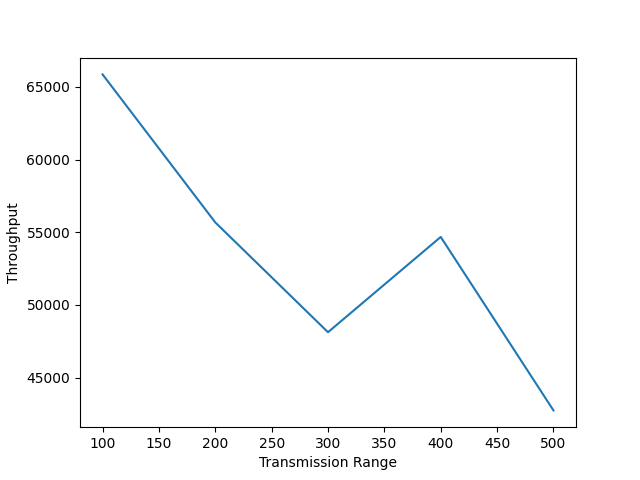
\includegraphics[width=.8\linewidth]{_15_4_static/TransmissionRangevsThroughput.png}
     \caption{Tx Range Vs Throughput}
    \label{tx_range_throughput}    
\end{subfigure}
\begin{subfigure}{.5\textwidth}
  \centering
  % include second image
  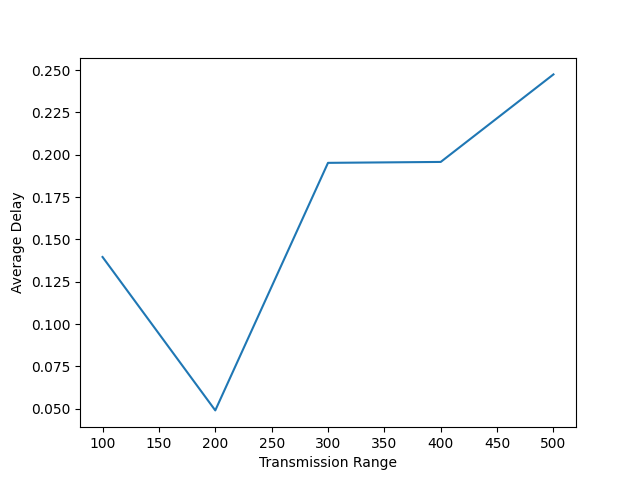
\includegraphics[width=.8\linewidth]{_15_4_static/TransmissionRangevsAverageDelay.png}
    \caption{Tx Range Vs Average Delay}
     \label{tx_range_delay}
\end{subfigure}
\begin{subfigure}{.5\textwidth}
  \centering
  % include third image
  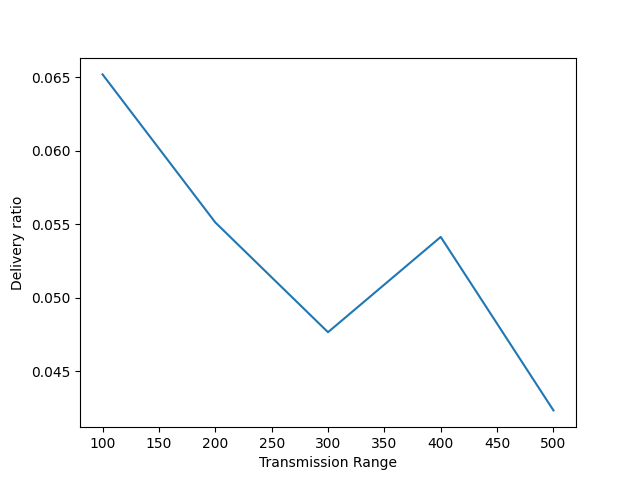
\includegraphics[width=.8\linewidth]{_15_4_static/TransmissionRangevsDeliveryRatio.png}
     \caption{Tx Range Vs Delivary Ratio}
     \label{tx_range_delivery}
\end{subfigure}
\begin{subfigure}{.5\textwidth}
  \centering
  % include fourth image
  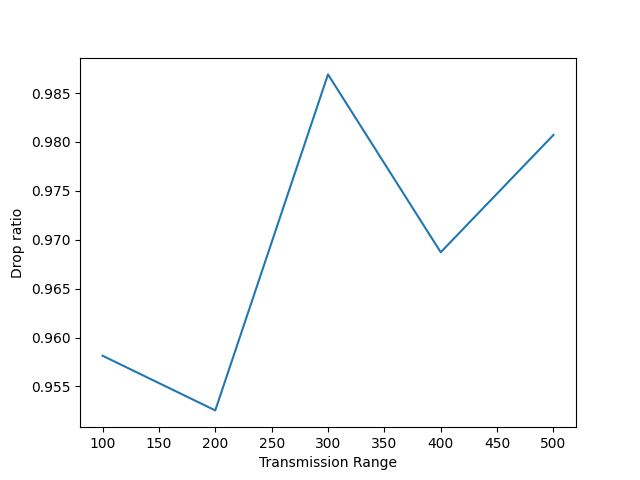
\includegraphics[width=.8\linewidth]{_15_4_static/TransmissionRangevsDropRatio.png}
     \caption{Tx Range Vs Drop Ratio}
     \label{tx_range_drop}
\end{subfigure}
\begin{subfigure}{.5\textwidth}
  \centering
  % include fifth image
  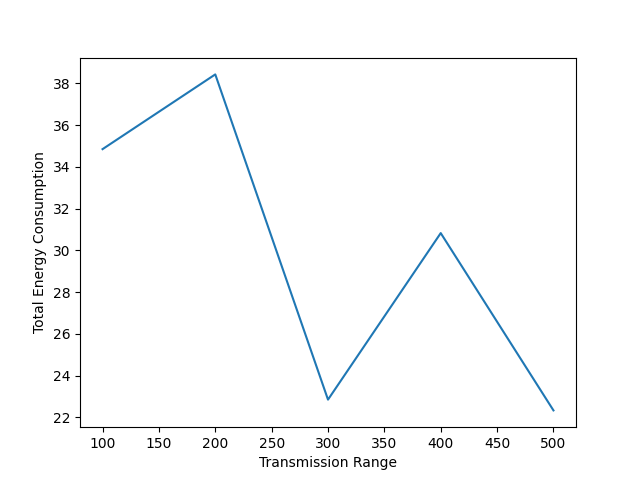
\includegraphics[width=.8\linewidth]{_15_4_static/TransmissionRangevsTotalEnergyConsumption.png}
     \caption{Tx Range Vs Energy Consumption}
     \label{tx_range_energy}
\end{subfigure}
\begin{subfigure}{.5\textwidth}
  \centering
  % include sixth image
  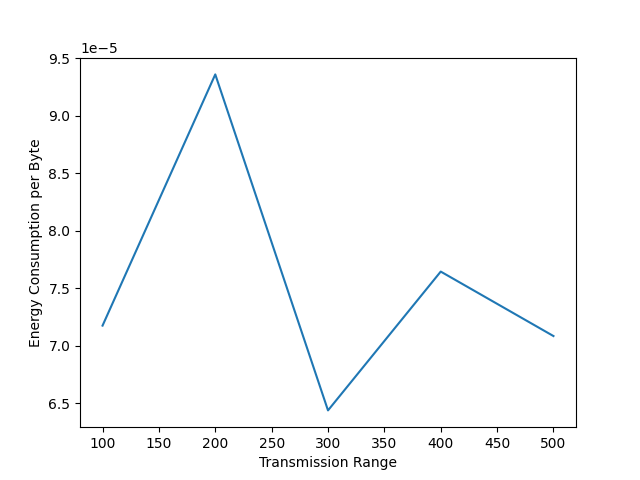
\includegraphics[width=.8\linewidth]{_15_4_static/TransmissionRangevsEnergyConsumptionperByte.png}
     \caption{Tx Range Vs Energy Per Byte}
     \label{tx_range_energy_per_byte}
\end{subfigure}
\caption{Varying Transmission Range}
\label{fig:varyingTxRange}
\end{figure}
\begin{figure}[h]
\begin{subfigure}{.5\textwidth}
  \centering
  % include first image
  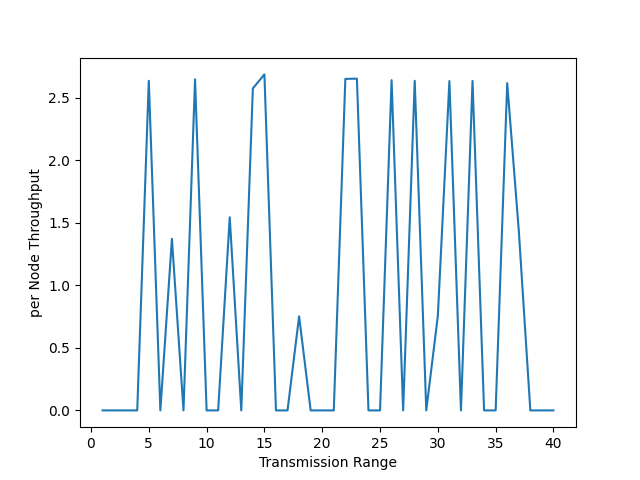
\includegraphics[width=.8\linewidth]{_15_4_static/TransmissionRange(100)vsperNodeThroughput.png}
     \caption{Tx Range(100) Vs Throughput per Node}
 \end{subfigure}
\begin{subfigure}{.5\textwidth}
  \centering
  % include second image
  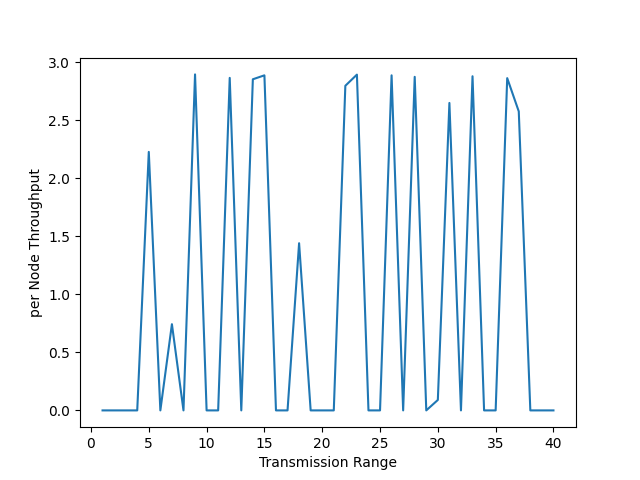
\includegraphics[width=.8\linewidth]{_15_4_static/TransmissionRange(200)vsperNodeThroughput.png}
     \caption{Tx Range(200) Vs Throughput per Node}
    \end{subfigure}
\begin{subfigure}{.5\textwidth}
    \centering
    % include third image
    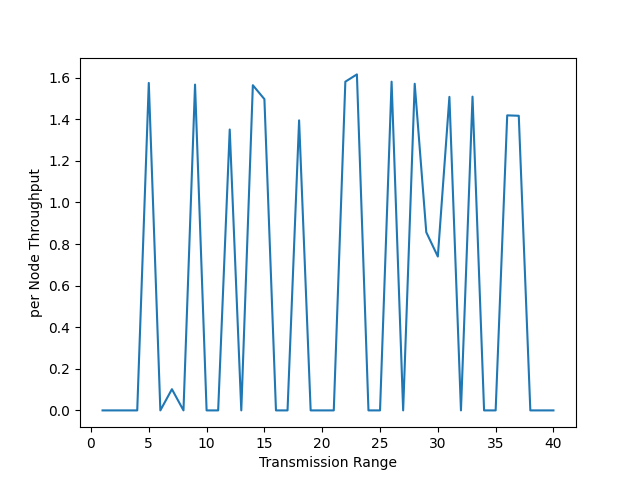
\includegraphics[width=.8\linewidth]{_15_4_static/TransmissionRange(300)vsperNodeThroughput.png}
         \caption{Tx Range(300) Vs Throughput per Node}
        \end{subfigure}
\begin{subfigure}{.5\textwidth}
    \centering
    % include fourth image
    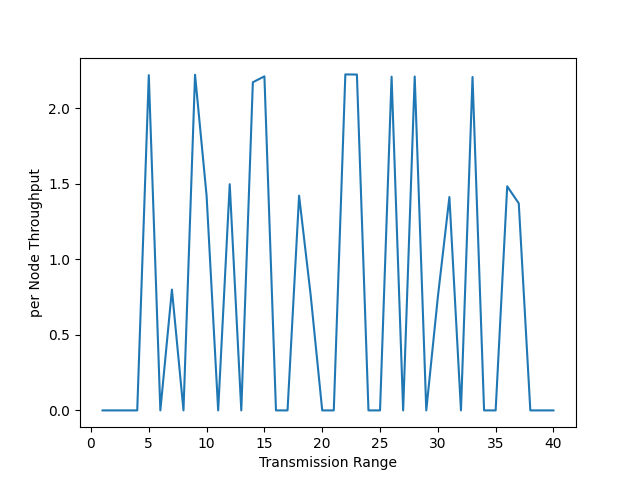
\includegraphics[width=.8\linewidth]{_15_4_static/TransmissionRange(400)vsperNodeThroughput.png}
         \caption{Tx Range(400) Vs Throughput per Node}
        \end{subfigure}
\begin{subfigure}{.5\textwidth}
    \centering
    % include fifth image
    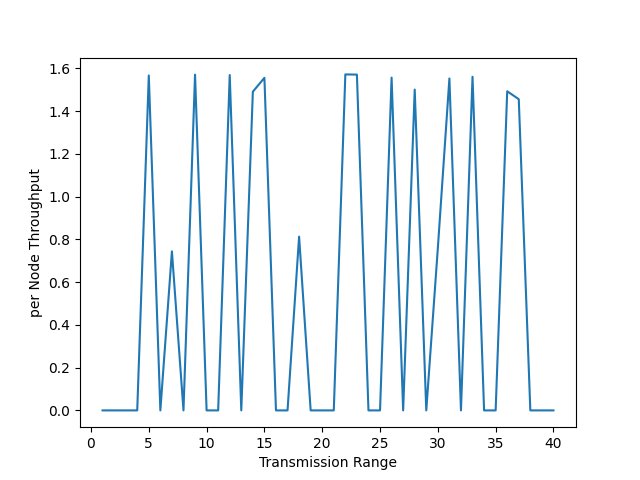
\includegraphics[width=.8\linewidth]{_15_4_static/TransmissionRange(500)vsperNodeThroughput.png}
         \caption{Tx Range(500) Vs Throughput per Node}
        \end{subfigure}
\caption{Varying Transmission Range (Throughput per Node)}
\label{tx_range_per_node_throughput}
\end{figure}

